\documentclass[convert={density=1000,size=600, outext=.png}]{standalone}
\usepackage{tikz}
\usetikzlibrary{arrows.meta, decorations.pathmorphing}
\begin{document}
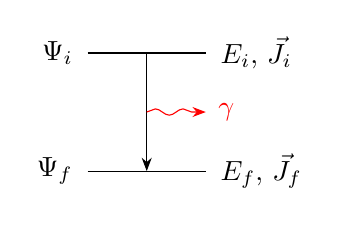
\begin{tikzpicture}[scale=3, >= Stealth]
  \draw (-0.25, 0.25)  -- (0.25, 0.25);
  \draw (-0.26, 0.25) node [left=1pt] {$\Psi_{i}$};
  \draw (0.26, 0.25) node [right=1pt] {$E_{i}$, $\vec{J}_{i}$};
  \draw (-0.26, -0.25) node [left=1pt] {$\Psi_{f}$};
  \draw (0.26, -0.25) node [right=1pt]{$E_{f}$, $\vec{J}_{f}$};
  \draw (-0.25, -0.25)-- (0.25, -0.25);
  \draw [->] (0, 0.25) -- (0, -0.25);
  \draw [red, ->, decorate, decoration={snake, amplitude=.4mm, post length=1mm}] (0, 0) -- (0.25, 0) node [right=1pt] {$\gamma$};
\end{tikzpicture}
\end{document}
